\documentclass{article}
\usepackage{tikz}

\begin{document}

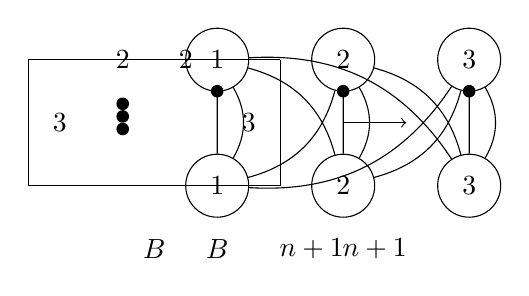
\begin{tikzpicture}[scale=0.8]
    % Left part of the image
    \draw (0,0) -- (4,0);
    \draw (0,2) -- (4,2);
    \draw (0,0) -- (0,2);
    \draw (4,0) -- (4,2);
    
    \node at (0.5, 1) {$3$};
    \node at (3.5, 1) {$3$};
    \node at (1.5, 2) {$2$};
    \node at (2.5, 2) {$2$};
    
    \foreach \x in {1,...,3} {
        \fill (1.5, 1.5 - \x * 0.2) circle (0.1);
    }
    
    \node at (2, -1) {$B$};
    \node at (3, -1) {$B$};
    
    % Right part of the image
    \draw[->] (5,1) -- (6,1);
    
    \foreach \x in {1,2,3} {
        \node[circle, draw, minimum size=0.8cm] (n\x) at (\x*2+1, 2) {\x};
    }
    
    \foreach \x in {1,2,3} {
        \node[circle, draw, minimum size=0.8cm] (m\x) at (\x*2+1, 0) {\x};
    }
    
    \foreach \x in {1,2,3} {
        \draw (n\x) -- (m\x);
    }
    
    \foreach \x in {1,2,3} {
        \foreach \y in {1,2,3} {
            \draw (n\x) to[bend left=30] (m\y);
        }
    }
    
    \node at (4.5, -1) {$n+1$};
    
    \foreach \x in {1,2,3} {
        \fill (\x*2+1, 1.5) circle (0.1);
    }
    
    \node at (5.5, -1) {$n+1$};
\end{tikzpicture}

\end{document}